Seit Ende des 19.~Jahrhunderts wird nun der Begriff der Radioaktivität untersucht, dessen Effekte zuerst 1896 durch Becquerel entdeckt und anschließend durch Marie und Pierre Curie untersucht wurden. Heute weiß man, dass es sich bei Radioaktivität um das Zerfallen instabiler Atomkernen handelt, welche beim Zerfallsprozess abstrahlen (radioaktive Strahlung). Mitunter, da die Strahlung zu massiven Gesundheitsschäden an sämtlichen Lebensformen nehmen kann, ist die Abschirmung dieser Strahlung von großer Bedeutung. Weiter ist auch die Messbarkeit radioaktiver Strahlung wichtig, da der Mensch diese nicht wahrnehmen kann. Beide Aspekte sind Teil dieses Versuchs. \cite{HW03}

\section{Aufbau der Atome}

\begin{figure}[tb]
	\centering
	
	\begin{subfigure}[b]{0.3\textwidth}
		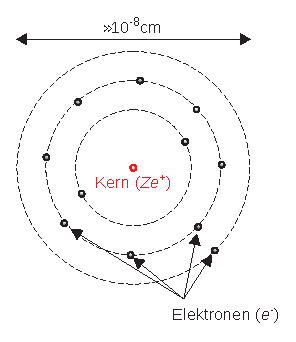
\includegraphics[width=\textwidth]{fig/i_01_atom.eps}
		\caption{}
		\label{fig:i_01_atom}
	\end{subfigure}
	\qquad\qquad\qquad\qquad
	\begin{subfigure}[b]{0.3\textwidth}
		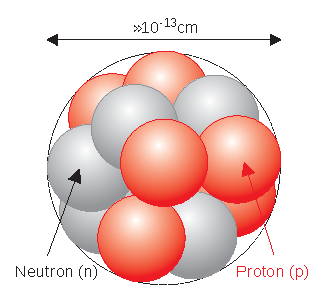
\includegraphics[width=\textwidth]{fig/i_02_kern.eps}
		\caption{}
		\label{fig:i_01_kern}
	\end{subfigure}
	
	\caption{(a) Aufbau eines Atoms; (b) Aufbau eines Atomkerns (aus \cite[S. 507]{EKS07}).}
\end{figure}

Die Materie, wie wir sie kennen, besteht aus Molekülen und Atomen, wobei die Moleküle selbst wieder Atome enthalten. Ein einzelnes Atom setzt sich aus einem elektrisch positiv geladenen Kern und mehreren negativ geladenen Elektronen zusammen. Die Elektronen sind sehr viel (ca. \nicefrac{1}{2000}-mal) leichter als der Kern. In klassischer Näherung umkreisen die Elektronen den Kern (s. Abb. \ref{fig:i_01_atom}). (Diese Anschauung ist allerdings nicht konsistent zur klassischen Elektrodynamik, laut welcher die Elektronen kontinuierlich Energie abstrahlen und somit in den Kern stürzen müssten. Das Atom wäre somit instabil; als erste anschauliche Vorstellung genügt es jedoch meist.) In der Quantenmechanik stellt man fest, dass die Elektronen eine gewisse Aufenthaltswahrscheinlichkeit um den Kern haben. In jedem Fall befinden sich die Elektronen in einem gewissen Bereich um den Kern, dessen halber Durchmesser als Atomradius bezeichnet wird. Dieser befindet sich in der Größenordnung von $\SI{1}{\angstrom}$. Die positive Ladung des Kerns ist ein vielfaches der Elementarladung (der Ladung eines Elektrons), $q = Z \cdot e$. Das Atom ist neutral geladen, wenn es genau so viele Elektronen in seiner Hülle bindet, wie es positive Ladungen in seinem Kern trägt. Andernfalls nennt man es ein Ion. Die Anzahl der Kernladungen ist charakteristisch für ein Atom und von maßgeblicher Bedeutung für die Chemie. Einzig durch die Wechselwirkung der Elektronen in der Hülle des Atoms mit denen anderer Atome kommt es zu chemischen Reaktionen und chemischen Bindungen. Der Kern spielt in diesem Teilbereich keine Rolle.\\
Der Kern (s. Abb. \ref{fig:i_01_kern}) besteht aus positiv geladenen Protonen und neutral geladenen Neutronen; sie zusammen bilden die so genannten Nukleonen. Die Elektrodynamik verbietet ein solches System zunächst, da die positiven Ladungen eine repulsive Kraft aufeinander ausüben. Es gibt jedoch eine weitere Kraft (die Kernkraft), welche zum Einen sehr stark ist, insbesondere stark genug, um die Protonen sehr nah beieinander zu halten, zum Anderen aber sehr lokalisiert ist, da sie nicht ausreicht, um auch die Nukleonen anderer Atomkerne anzuziehen. Im Rutherfordschen Streuexperiment wird die Streuung von vollständig ionisierten Helium-Atomen an einer Goldfolie untersucht. Wegen des Coulomb-Potentials des quasi punktförmigen Kerns des Gold-Atoms bewegt sich der Helium-Kern auf einer Hyperbel am Gold-Kern vorbei. Je größer die Energie der eingestrahlten Teilchen ist, desto geringer ist der minimale Abstand zwischen Projektil und Target, der erreicht wird. Ab einer bestimmten Energie bricht die Transmission ein, die Helium-Kerne werden von den Gold-Kernen absorbiert. Aus der Energie der Teilchen lässt sich berechnen, ab welchem Radius die Teilchen absorbiert werden. Ab diesem Abstand erfahren die Helium-Kerne attraktive Wechselwirkungen durch die Kernkräfte. Dieser Abstand wird auch als Kernradius bezeichnet und befindet sich in der Größenordnung von $\SI{1}{fm}$, ist also sehr viel kleiner als der Atomradius. \cite{HW03}\\
Die Protonen und Neutronen im Kern haben ungefähr die Gleiche Masse,
\begin{equation}
m_\textrm n \approx m_\textrm p = \SI{1,67E-27}{kg} \approx 1836 \cdot m_\textrm e.
\end{equation}
Als Massenzahl $A \in \mathbb{N}$ definiert man die Anzahl der Nukleonen, also die Summe der Anzahl der Protonen (Ordnungszahl) $Z$ und der Neutronen $N$,
\begin{equation}
A = Z + N.
\end{equation}
Die Zahl der Protonen $Z$ definiert, um welches chemisches Element es sich handelt (Position im Periodischen System der Elemente). Atome des gleichen chemischen Elementes mit unterschiedlichen Neutronen-Zahlen bezeichnet man als Isotope. Zur Kennzeichnung einer bestimmten Sorte von Atomen wird die Zahl der Protonen $Z$ und die Massenzahl $A$ vor die Abkürzung des Elements geschrieben, z.B. bezeichnet $\element{C}{6}{12}$ den Kohlenstoff mit $6$ Protonen und $6$ Neutronen.\\
Nicht alle Atomkerne sind stabil (Radionuklide). Es gibt Elemente mit stabilen Isotopen (jene geringer Ordnungszahl) und Elemente ohne ein stabiles Isotop (jene hoher Ordnungszahl). Jedes Element weist jedoch eine instabile Konfiguration auf. Ist ein Kern instabil, so zerfällt er. Mit stabilen und instabilen Kernen können außerdem Kernfusion und Kernspaltung durchgeführt werden. Bei der Kernspaltung teilt sich der Kern in zwei Elemente auf; bei der Kernfusion entsteht aus zwei Kernen ein neuer Kern.\\
Der Zerfall von Kernen lässt sich im Widerspruch zur klassischen Physik nicht voraussagen. Es lässt sich lediglich eine Halbwertszeit $T_{\nicefrac{1}{2}}$ für eine Zerfallsart eines Isotops messen. Diese gibt an, nach welcher Zeit nur noch die Hälfte der Isotope des untersuchten Elements vorhanden sind. Es lässt sich vor dem Zerfall jedoch nicht bestimmen, welche Atome zerfallen werden. Dies geschieht willkürlich und nur in der Gesamtheit lässt sich eine Aussage mittels der Halbwertszeit treffen. Der Zerfall der Atome lässt sich durch Einwirkungen von außen so gut wie nicht beeinflussen (außer man beschießt den Kern mit hochenergetischen Teilchen). Insbesondere haben chemische Bedingungen keine Effekte auf den Zerfall der Atome.\\

\section{Zerfall}
Instabile Kerne können zerfallen. Dabei ändert sich durch verschiedene Vorgänge ihre Massenzahl und/oder ihre Ordnungszahl. Meist handelt es sich nicht um einen einzigen Zerfallsprozess, sondern um eine Zerfallsreihe. Zerfällt ein instabiles Isotop in ein anderes, so zerfällt dieses weiter, bis ein stabiles Isotop erreicht wird. Manche Isotope können auf unterschiedlichen Weise zerfallen und sich so in verschiedene Elemente umwandeln. Es entstehen viele verschiedene parallel ablaufende Zerfallsreihen. Zunächst zu den möglichen Zerfallsarten:
\begin{itemize}
 \item{\textbf{$\upalpha$-Zerfall:}} Ein instabiler Kern kann unter Aussendung eines vollständig ionisierten Helium-Kerns ($\alpha$-Teilchen) seine Massenzahl um $4$ und seine Ordnungszahl um $2$ verringern.
 \item{\textbf{$\upbeta^-$-Zerfall:}} Hierbei wandelt sich im Kern ein Neutron in ein Proton um. Es verändert sich die Massenzahl also nicht, die Ordnungszahl jedoch steigt. Dabei wird ein Elektron und ein Elektron-Anti-Neutrino erzeugt und mit der freigesetzten Energie aus dem Kern gestrahlt.
 \item{\textbf{$\upbeta^+$-Zerfall:}} Diese läuft analog zur $\upbeta^-$-Zerfall ab, jedoch verläuft hier die Umwandlung umgekehrt. Es wird also ein Proton in ein Neutron umgewandelt, so verringert sich die Ordnungszahl um 1. Die entstehenden Teilchen sind dabei ein Anti-Elektron (oder auch Positron) und ein Elektron-Neutrion.
\end{itemize}
Die Zerfälle können durch die Fajans-Soddyschen Verschiebungsgesetze dargestellt werden:
\begin{equation}
\element{X}{A}{Z} \xrightarrow{\upalpha} ~~\element{X'}{A - 4}{Z - 2},\qquad \element{Y}{A}{Z} \xrightarrow{\upbeta^-} ~~\element{Y'}{A}{Z + 1},\qquad \element{Y}{A}{Z} \xrightarrow{\upbeta^+} ~~\element{Y'}{A}{Z - 1}
\end{equation}
Bei den oben genannten Zerfällen entstehen entsprechende gleichnamige Strahlungen. Neben der ausgesandten Teilchen wird Energie in Form von elektromagnetischer Strahlung frei gesetzt. Diese sehr hochenergetische Strahlung nennt sich auch $\gamma$-Strahlung, welche bei vielen Prozessen zusätzlich entsteht. Die Strahlungsarten unterscheiden sich mit unter wesentlich durch ihre Durchdringungsfähigkeit der Materie. Die abgestrahlten Teilchen ionisieren Atome in der umgebenden Materie und verlieren dabei an Energie. Je mehr ein Teilchen auf einem Raumbereich ionisiert, desto geringer ist die Durchdringungsfähigkeit. Diese hängt natürlich auch vom zu durchdringenden Material, insbesondere von dessen Dichte, ab. Auch das Gewicht der wechselwirkenden Teilchen ist wichtig, da die Strahlung mehr Energie an Teilchen gleicher Masse verlieren kann.\\
$\upalpha$-Teilchen wechselwirken sehr stark und haben daher eine nur sehr kurze Reichweite. $\upbeta^-$- und $\upbeta^+$-Teilchen haben eine höhere Reichweite und wechselwirken deutlich weniger mit der Umgebung. Die $\upgamma$-Strahlung hingegen wechselwirkt nur sehr wenig und hat eine sehr hohe Reichweite.\\
Bei den Umwandlungsprozessen wird eine feste, diskrete Energie frei gesetzt. Beim $\upalpha$-Zerfall wird diese Energie auf das $\upalpha$-Teilchen übertragen und dieses hat für jeden Zerfall dieser Sorte einen festen Wert. Bei den $\upbeta$-Zerfällen sind hingegen zwei Teilchen im Spiel, unter welchen sich die Energie des Zerfalls aufteilt. Somit findet man bei ein und dem gleichen $\upbeta$-Zerfall Strahlung unterschiedlicher Energie. Da die Energie des Elektron-Neutrinos minimal 0 werden kann, gibt es für das Elektron und somit die $\upbeta^-$-Strahlung eine maximale Energie. \cite{EKS07}

\section{Geiger-Müller-Zählrohr}
Das Geiger-Müller-Zählrohr nutzt die ionisierende Wirkung der radioaktiven Strahlung aus, um diese zu messen. Es handelt sich um ein mit Gas gefülltes zylindrisches Gefäß, in dessen Mitte axial ein Draht geführt wird (s. Abb. \ref{fig:i_03_geigermueller}). Zwischen Draht und Gefäßwand wird eine Spannung angelegt. Ionisiert radioaktive Strahlung die Gasmoleküle, werden diese zu den entsprechenden Leitern hin beschleunigt. Aufgrund der Beschleunigung erhalten die Ionen und die Elektronen zwischen den Stößen mit anderen Gas-Teilchen so viel Energie, dass sie es schaffen, andere Moleküle und Atome zu ionisieren. Es entsteht ein Lawinen-Effekt, welcher zu einem messbaren Stromfluss führt. Anhand dessen kann das Eintreten eines radioaktiven Strahlteilchens registriert werden.\\
Treten mehrere Teilchen in kurzer Zeit nacheinander in das Zählrohr ein, kann das nachfolgende Teilchen eventuell nicht registriert werden. Grund ist die Abschirmung des elektrischen Feldes in der Gaskammer durch die Ionen des zuvor registrierten Teilchens. Die Zeit, in der das Rohr daher keine weiteren Teilchen registrieren kann, nennt man Totzeit $t_\mathrm{tot}$ und ist bei den meisten Zählrohren in der Größenordnung von $\SI{1}{ms}$.

\begin{figure}[tb]
\centering
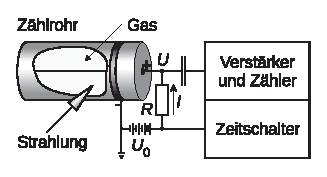
\includegraphics{fig/i_03_geigermueller.eps}
\caption{Aufbau eines Geiger-Müller-Zählrohrs (aus \cite[S. 514]{EKS07}).}
\label{fig:i_03_geigermueller}
\end{figure}

Untersucht man die registrierten Teilchen des Zählrohrs als Funktion der Spannung bei konstanter Einstrahlung, findet man folgenden Zusammenhang: Bis zu einem Schwellwert $U_\mathrm S$ reicht die Spannung nicht aus, um einen Kaskaden-Effekt zur erreichen, man misst also keine Registrierungen. Danach wächst die Zählrate mit der Spannung an. Man erreicht einen Bereich, in dem jedes eintreffende ionisierende Teilchen registriert wird, den Plateau-Bereich. In diesem Bereich ändert sich die Zählrate nur wenig. Erhöht man die Spannung weiter, kommt es zu Dauergasentladung, welche das Zählrohr ggf. sogar zerstören kann (s. Abb. \ref{fig:i_04_kennlinie}).

\begin{figure}[tb]
\centering
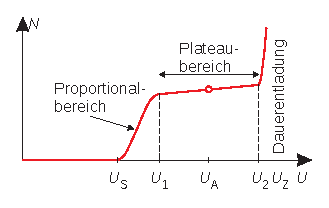
\includegraphics[]{fig/i_04_kennlinie.eps}
\caption{Kennlinie eines Geiger-Müller-Zählrohrs (aus \cite[S. 515]{EKS07}).}
\label{fig:i_04_kennlinie}
\end{figure}

Neben der untersuchten Strahlung (bspw. die einer radioaktiven Probe) gibt es ständig eine nicht vermeidbare Zählrate, die sogenannte Nullrate $N_0$. Sie wird durch die Strahlung radioaktiver Verunreinigungen in der vom Versuchsaufbau umgebenden Materie oder durch kosmische Strahlung verursacht. Sie sollte bei der Untersuchung von Strahlungen stets mit berücksichtigt werden.
\begin{equation}
N_{\mathrm{ges}} = N_\mathrm{P} + N_0.
\end{equation}
Bei der Abschirmung von Strahlung ist generell noch zu beachten, dass die Strahlung gemäß des $\nicefrac{1}{r^2}$-Abstandsgesetzes abnimmt. Der Abstand der Probe zum Zählrohr ist damit - unabhängig von der Durchdringungsfähigkeit der Strahlung - maßgeblich für die Zahl der gemessenen Registrierungen. \cite{EKS07}